\documentclass[conference]{IEEEtran}
\usepackage{amsmath,amssymb,booktabs,graphicx}
\usepackage[hidelinks]{hyperref}
\graphicspath{{results/analysis/}{../../results/analysis/}}
\title{Systolic Array Scaling Under Modeled Input Bandwidth Limits}
\author{\IEEEauthorblockN{Ozlem Polat, Thomas Martin, and Keith Kamer}
\IEEEauthorblockA{University of Florida\\EEL5764 Computer Architecture, Fall 2026}}
\begin{document}
\maketitle
\begin{abstract}
We evaluate a parameterized output-stationary VHDL matrix multiplier across three processing-element grids, two matrix orders, and three modeled operand-supply budgets. All 18 configurations pass eight full-width correctness cases, independently rerun using GHDL after the original Questa evaluation. For order-16 products at full supply, the 2-by-2, 4-by-4, and 8-by-8 arrays require 1216, 368, and 124 compute clocks. The largest array achieves 9.806 times the baseline speedup using 16 times as many processing elements. Limiting that array to four combined input words per clock introduces 180 stalls and raises latency to 304 clocks. A cycle decomposition identifies budget stalls, fill/drain, and per-tile capture costs. The available 2-by-2 FPGA result uses four DSPs and meets its internal 10 ns constraint. Larger-grid FPGA measurements remain pending in this draft; hardware scaling conclusions are withheld until they are available.
\end{abstract}
\begin{IEEEkeywords}
systolic array, matrix multiplication, input bandwidth, FPGA, architectural evaluation
\end{IEEEkeywords}

\section{Research Question and Scope}
More arithmetic resources do not guarantee proportional performance improvement if operand delivery or finite-workload overhead prevents useful utilization. We ask how grid dimension and a controlled input-supply budget affect the latency, useful throughput, utilization, and FPGA implementation cost of one complete matrix multiplier.

We compare square processing-element (PE) grids of dimension $P\in\{2,4,8\}$, square matrix orders $N\in\{8,16\}$, and combined input budgets $B\in\{4,8,16\}$ words per clock. All configurations compute the same complete product for a given workload. The input budget is a modeled RTL interface limit; the study does not measure physical KV260 memory bandwidth. There is no processor interface, external DRAM controller, alternate dataflow, CPU baseline, power measurement, or required board demonstration.

The baseline is the 2-by-2 grid. We hypothesize that input limitations reduce larger-grid scaling efficiency and that short products retain significant fill/drain overhead even at full supply. The experiments need not show a complete scaling plateau to answer these questions.

\section{Implemented Architecture}
Each PE receives a signed 16-bit $A$ operand from the left and a signed 16-bit $B$ operand from above. Registered links forward operands and associated valid bits. When both operands are valid on an enabled edge, the PE accumulates their signed product into a local 36-bit result:
\begin{equation}
 C[i,j]=\sum_{k=0}^{N-1} A[i,k]B[k,j].
\end{equation}
The width preserves the exact 16-term sum, including repeated products of $-32768$ with itself. The output remains stationary while operands move through the array.

For an output tile at $(r_0,c_0)$, the controller injects $A[r_0+r,k]$ on boundary step $k+r$ and $B[k,c_0+c]$ on step $k+c$. They meet at PE $(r,c)$ on enabled step $k+r+c$. All grid state holds during a budget stall, preserving alignment.

When $N>P$, the controller visits $(N/P)^2$ output tiles in row-major order. Every tile streams the full inner dimension $N$. A capture clock stores its $P^2$ results and clears the grid. The complete result is subsequently read serially in $N^2$ clocks. The readout interface has no backpressure and assumes every valid word is consumed.

The input stager accepts at most $B$ new boundary words per clock, retaining accepted values while a step is incomplete. It bypasses unstored values on the completing clock, avoiding an artificial staging clock at full supply. Empty drain steps advance normally. Optional counters and debug outputs are disabled by the synthesis generic \texttt{INSTR=false}; an RTL regression checks agreement with the instrumented datapath.

\section{Methodology and Validation}
The Cartesian product gives 18 architectural configurations. Each is evaluated using zero, identity, two signed-extreme, mixed-sign, and three fixed-seed random cases. An independent Python matrix multiplication produces exact reference results. The vector manifest records the seed, case order, and canonical LF-byte SHA-256 hashes.

The original QuestaSim 2026.2 sweep records 144 passing cases. The follow-up GHDL sweep independently verifies the same cases, comparing every output at full 36-bit width, requiring exactly $N^2$ ordered result words and $N^3$ useful MACs. Counter formulas are supplemented by independent interface-clock observations. Directed tests cover reset/clear priority, stall hold, valid forwarding, partially staged words, sparse/empty steps, and the synthesis instrumentation setting. CI repeats these checks for future pull requests and retains logs and measurements.

Compute latency begins with the first accepted input and ends at the final tile capture. It includes staging, budget stalls, fill/drain, and tile transitions. Total latency adds serial readout. Useful throughput and utilization are
\begin{align}
 T_{\mathrm{MAC}} &= N^3/C_{\mathrm{compute}},\\
 U_{\mathrm{PE}} &= N^3/(P^2 C_{\mathrm{compute}}).
\end{align}
Speedup divides the 2-by-2 latency by candidate latency for identical $N$, $B$, and inputs. Scaling efficiency divides speedup by $P^2/4$.

Vivado 2025.2.1 performs out-of-context synthesis, optimization, placement, and routing for part \texttt{xck26-sfvc784-2LV-c}, using a common 10 ns clock constraint. Only P=2/N=16 reports are currently available. The remaining grids must use comparable source and settings.

\section{Cycle Accounting}
Let $Q=(N/P)^2$ denote output tiles. Each tile advances for $N+2P-2$ enabled steps and uses one capture clock. Boundary step $t$ requires
\begin{equation}
 w(t)=2\left|\{i:0\leq i<P,\ 0\leq t-i<N\}\right|
\end{equation}
new words. The budget stall count is
\begin{equation}
 S=Q\sum_{t=0}^{N+2P-3}\max\left(0,\left\lceil w(t)/B\right\rceil-1\right).
\end{equation}
The implemented latency is
\begin{align}
 C_{\mathrm{compute}} &= QN+Q(2P-2)+Q+S,\\
 C_{\mathrm{total}} &= C_{\mathrm{compute}}+N^2.
\end{align}
$QN=N^3/P^2$ is useful-equivalent work normalized by peak PE capacity. This decomposition does not imply that useful MACs occur in a separate interval: useful work overlaps fill/drain. The independent model validates actual measured counters; it does not substitute predicted results for missing runs.

\begin{figure*}[t]
\centering
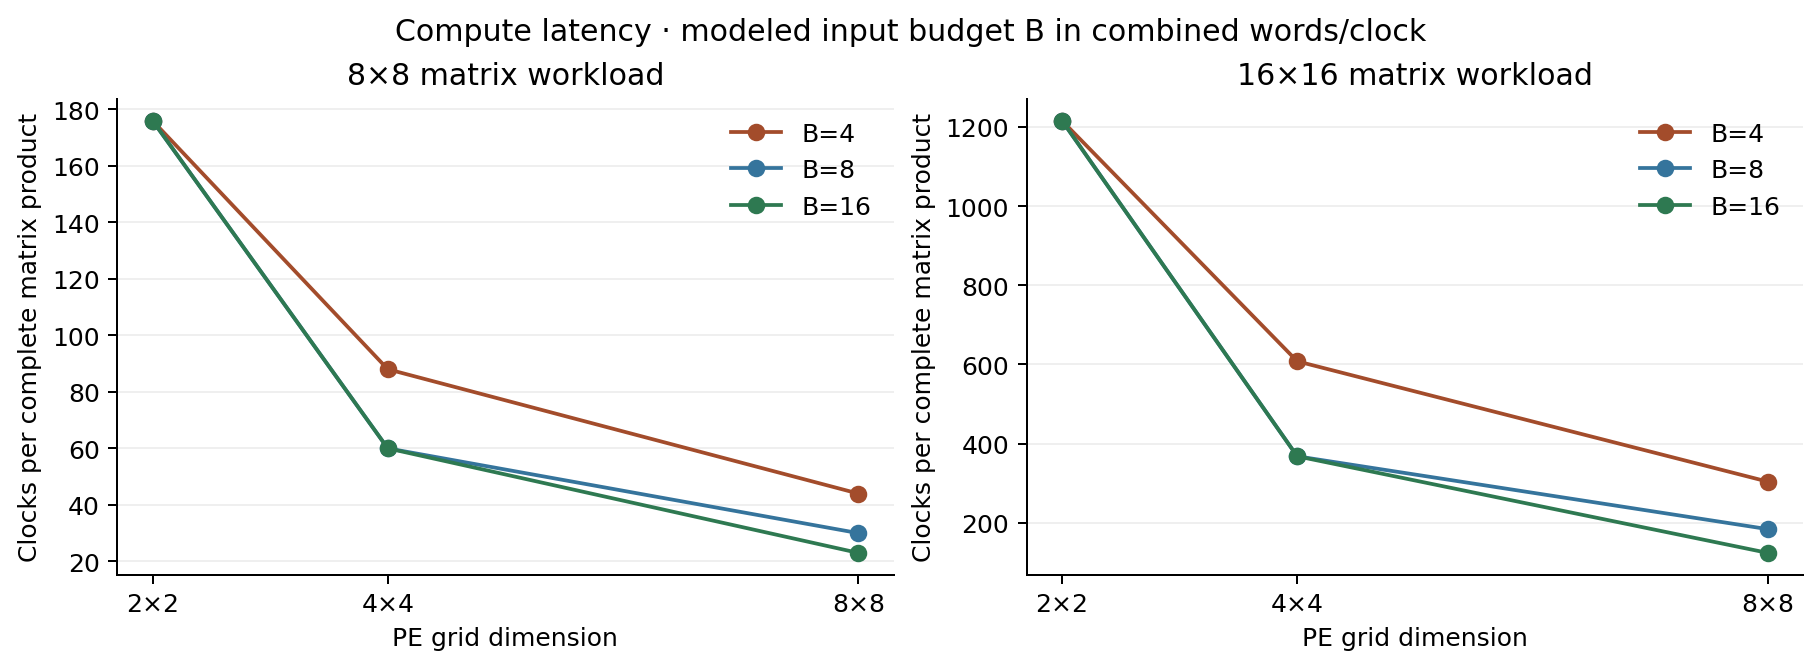
\includegraphics[width=\textwidth]{latency.png}
\caption{Measured compute latency across grid dimensions, workloads, and modeled input budgets. All products are complete and numerically verified.}
\label{fig:latency}
\end{figure*}

\section{Measured Results and Interpretation}
At $N=16,B=16$, compute cycles are 1216, 368, and 124 for $P=2,4,8$. Speedups are 3.304 and 9.806 for the two larger grids, compared with ideal PE-count increases of four and sixteen. The largest grid therefore achieves 61.3\% scaling efficiency and 51.6\% useful utilization at full supply.

For $N=16,P=8$, reducing $B$ from sixteen to eight introduces 60 stalls and raises latency from 124 to 184 clocks. Reducing it to four introduces 180 stalls and raises latency to 304 clocks, a 2.452-fold latency increase. These measurements directly isolate the modeled supply penalty because the enabled-step and capture counts remain constant.

At full supply, the same product uses 64 useful-equivalent clocks, 56 fill/drain clocks, and four capture clocks. Thus finite-workload scheduling limits utilization even when no input stalls occur. The smaller $N=8,P=8,B=16$ product takes 23 compute clocks and 64 readout clocks, demonstrating why compute and end-to-end speedup must be reported separately.

\begin{table}[t]
\centering
\caption{Order-16 simulation measurements.}
\begin{tabular}{rrrrrr}
\toprule
$P$ & $B$ & Compute & Stalls & MACs/clock & Util. (\%)\\
\midrule
2 & 4/8/16 & 1216 & 0 & 3.368 & 84.2\\
4 & 4 & 608 & 240 & 6.737 & 42.1\\
4 & 8/16 & 368 & 0 & 11.130 & 69.6\\
8 & 4 & 304 & 180 & 13.474 & 21.1\\
8 & 8 & 184 & 60 & 22.261 & 34.8\\
8 & 16 & 124 & 0 & 33.032 & 51.6\\
\bottomrule
\end{tabular}
\end{table}

A larger array still improves compute latency in every tested configuration. At $B=4$, the 8-by-8 takes half the clocks of the 4-by-4 for both matrix orders. We therefore conclude that limited input supply reduces scaling efficiency; this sweep does not establish a point beyond which grid growth ceases to help.

\section{FPGA Evidence and Limitations}
The available post-route P=2/N=16 implementation uses 7260 LUTs, 9437 FFs, four DSPs, and zero BRAM, with +3.955 ns internal WNS at the 10 ns constraint. The $16\times16\times36$-bit result store maps to registers, accounting for 9216 storage bits. This is a measured mapping result, not a BRAM estimate.

\begin{table}[t]
\centering
\caption{Post-route FPGA evidence. Pending rows are not estimates.}
\begin{tabular}{rrrrrl}
\toprule
$P$ & LUTs & FFs & DSPs & BRAM & WNS (ns)\\
\midrule
2 & 7260 & 9437 & 4 & 0 & +3.955\\
4 & \multicolumn{5}{c}{Pending actual Vivado run}\\
8 & \multicolumn{5}{c}{Pending actual Vivado run}\\
\bottomrule
\end{tabular}
\end{table}

The original OOC report lists 71 input ports and 63 output ports without delay constraints. Positive WNS applies to constrained internal paths and does not establish board I/O timing, measured system throughput at 100 MHz, or an achievable unconstrained maximum frequency. FPGA cost scaling and throughput per DSP remain incomplete until the P=4/P=8 runs are collected. No power or energy conclusion is inferred from resource counts.

\section{Conclusion and Completion Gate}
The verified RTL study demonstrates two distinct sources of sublinear scaling: budget-induced grid holds and finite-workload fill/drain/capture overhead. More PEs improve every measured case, while improving supply from four to sixteen words substantially benefits the 8-by-8. The remaining experimental gate is comparable larger-grid post-route evidence. Before final submission, replace the explicitly pending FPGA rows, regenerate cost-normalized figures, and revise hardware conclusions to match those measurements.

\section*{Reproducibility and Contribution Record}
Source, fixed vectors, scripts, CI configuration, measured CSVs, and analysis figures are maintained at \url{https://github.com/OzPol/systolic-array-scaling}. Thomas Martin delivered the initial RTL, testbench, original Questa sweep, and P=2 Vivado evidence in commits \texttt{3459a9f} and \texttt{d771fc7}, merged separately through PR 1. Subsequent verification, analysis, CI, setup documentation, and regressions are recorded as separate follow-up commits. The report source is a draft until missing hardware evidence and rendered layout are reviewed.
\end{document}
